\documentclass{article}
\usepackage[T2A]{fontenc}
\usepackage[utf8]{inputenc}
\usepackage[russian]{babel}
\usepackage{amssymb,amsmath,amsthm}
\usepackage{systeme,mathtools}
\usepackage{lipsum}
\usepackage{relsize}
\newcommand\md{\ }
\usepackage[normalem]{ulem}
\usepackage{pdfpages}

\begin{document}
\selectlanguage{russian}

\includepdf[pages=-]{Ok.pdf}
\section{Задание}

1.Создать класс, описывающий модель окружности (Circle). В классе должны быть описаны нужные свойства окружности и методы для получения, изменения этих свойств. Протестировать работу класса в классе CircleTest, содержащим метод статический main(String[] args).

2.Создать класс, описывающий тело человека(Human). Для описания каждой части тела создать отдельные классы(Head, Leg, Hand). Описать необходимые свойства и методы для каждого класса. Протестировать работу класса Human.

3.Создать класс, описывающий книгу (Book). В классе должны быть описаны нужные свойства книги(автор, название, год написания и т. д.)и методы для получения, изменения этих свойств. Протестировать работу класса в классе BookTest, содержащим метод статический main(String[] args).

\section{Ход работы}

В ходе выполнения работы были получены следующие исходные коды:

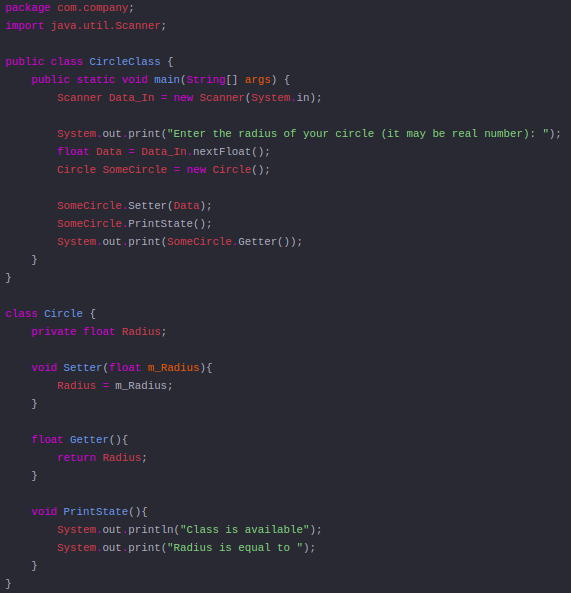
\includegraphics[width=0.85\linewidth]{view1.png}

\caption{Рисунок 1. Фрагмент кода для реализации задания с классом Circle.}

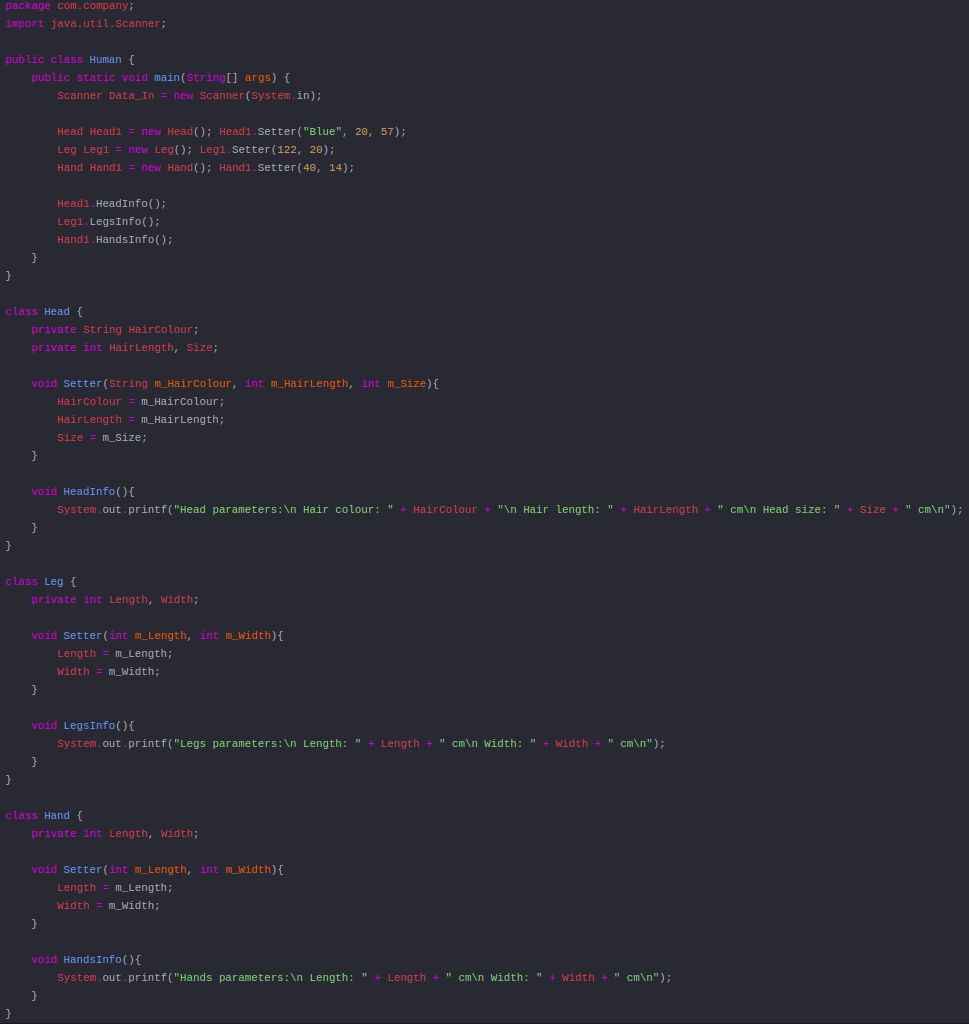
\includegraphics[width=1.2\linewidth]{view2.png}

\caption{Рисунок 2. Фрагмент кода для реализации задания с классом Human.}

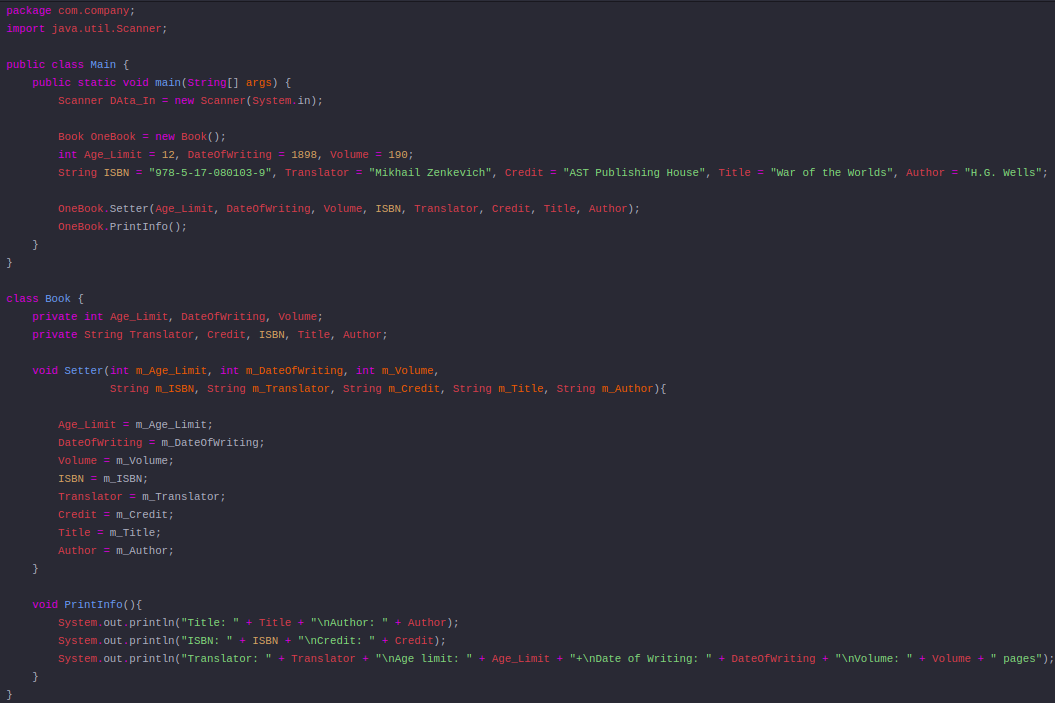
\includegraphics[width=1\linewidth]{view3.png}

\caption{Рисунок 3. Фрагмент кода для реализации задания с классом Book.}

\section{Вывод}
В ходе выполнения практического занятия номер 3 я научилась создавать классы с разнообразными методами и свойствами на языке программирования Java.

\end{document}
